
            \documentclass{article}
            \usepackage{tikz}
            \usepackage{xcolor}
            \usepackage{graphicx}
            \usepackage{caption}
    
            \definecolor{skyblue}{RGB}{135,206,235}
            \definecolor{brightmaroon}{RGB}{195, 33, 72}
    
            \usetikzlibrary{arrows.meta, shapes, positioning, matrix}
    
            \begin{document}
    
            \begin{figure}[htbp]
            \centering
            \resizebox{.45\linewidth}{!}{
            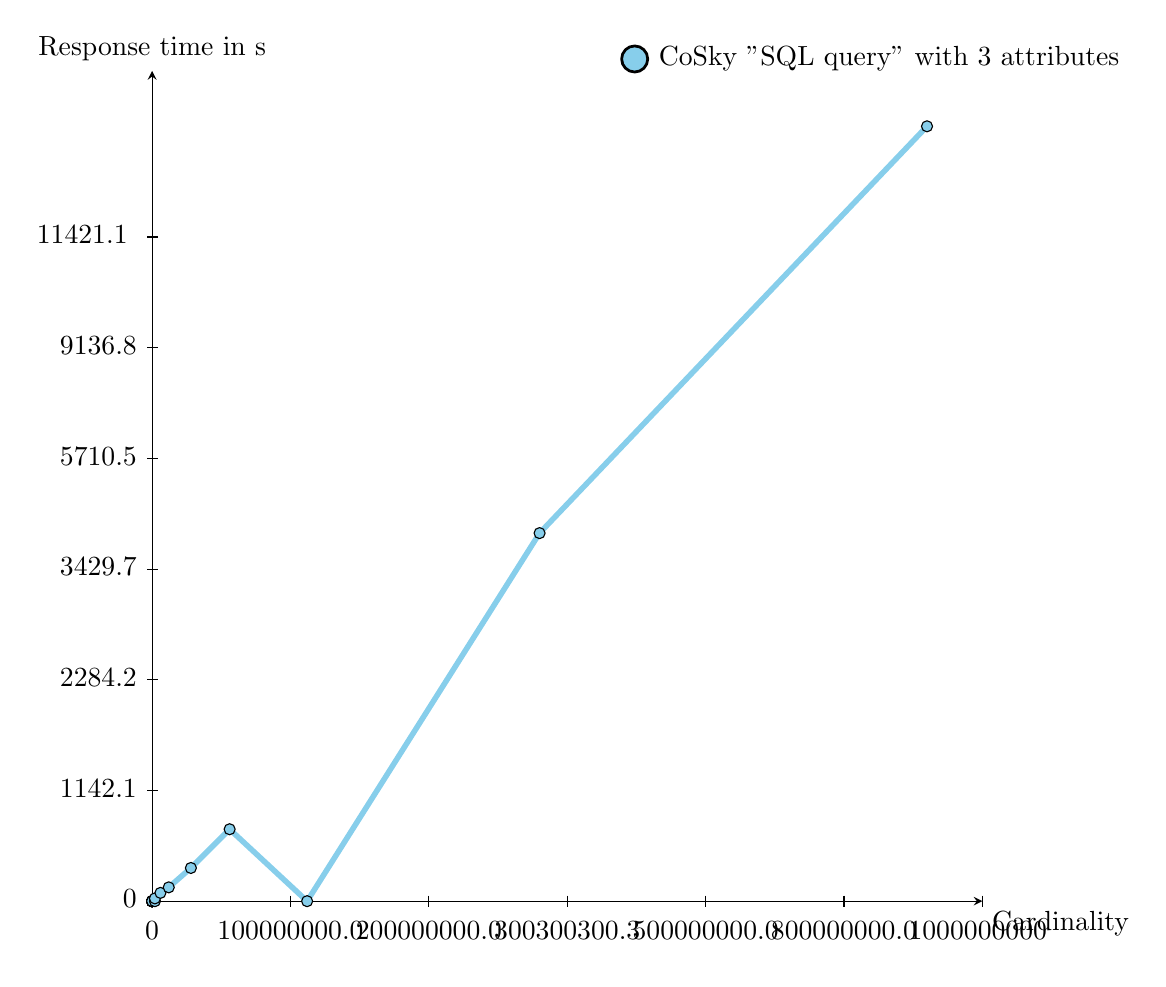
\begin{tikzpicture}[
            line join=bevel,
            bigcyannode/.style={shape=circle, fill=cyan, draw=black, line width=1pt},
            bigskybluenode/.style={shape=circle, fill=skyblue, draw=black, line width=1pt}
            ]
    
            % Axes
            \draw[-stealth] (0pt, 0pt) -- (300pt, 0pt) node[anchor=north west] {Cardinality};
            \draw[-stealth] (0pt, 0pt) -- (0pt, 300pt) node[anchor=south] {Response time in s};
            
            % X-axis ticks and labels
            \foreach \x/\xtext in {
                0pt/$0$,
                50pt/$100000000.0$,
                100pt/$200000000.0$,
                150pt/$300300300.3$,
                200pt/$500000000.0$,
                250pt/$800000000.0$,
                300pt/$1000000000$
            } {
                \draw (\x, 2pt) -- (\x, -2pt) node[below] {\xtext\strut};
            }
    
            % Y-axis ticks and labels
            \foreach \y/\ytext in {
                0pt/$0$,
                40pt/$1142.1$,
                80pt/$2284.2$,
                120pt/$3429.7$,
                160pt/$5710.5$,
                200pt/$9136.8$,
                240pt/$11421.1$
            } {
                \draw (2pt, \y) -- (-2pt, \y) node[left] {\ytext\strut};
            }
            \draw[skyblue, line width=2pt](0pt, 0pt) -- (0pt, 0pt) -- (0pt, 0pt) -- (0pt, 0pt) -- (0pt, 0pt) -- (0pt, 0pt) -- (0pt, 0pt) -- (0pt, 0pt) -- (0pt, 0pt) -- (0pt, 0pt) -- (0pt, 0pt) -- (0pt, 0pt) -- (0pt, 0pt) -- (0pt, 0pt) -- (0pt, 0pt) -- (0pt, 0pt) -- (1pt, 0pt) -- (1pt, 1pt) -- (3pt, 3pt) -- (6pt, 5pt) -- (14pt, 12pt) -- (28pt, 26pt) -- (56pt, 0pt) -- (140pt, 133pt) -- (280pt, 280pt);
% Points and labels
\filldraw[color=black, fill=skyblue] (0pt, 0pt) circle (2pt);
\filldraw[color=black, fill=skyblue] (0pt, 0pt) circle (2pt);
\filldraw[color=black, fill=skyblue] (0pt, 0pt) circle (2pt);
\filldraw[color=black, fill=skyblue] (0pt, 0pt) circle (2pt);
\filldraw[color=black, fill=skyblue] (0pt, 0pt) circle (2pt);
\filldraw[color=black, fill=skyblue] (0pt, 0pt) circle (2pt);
\filldraw[color=black, fill=skyblue] (0pt, 0pt) circle (2pt);
\filldraw[color=black, fill=skyblue] (0pt, 0pt) circle (2pt);
\filldraw[color=black, fill=skyblue] (0pt, 0pt) circle (2pt);
\filldraw[color=black, fill=skyblue] (0pt, 0pt) circle (2pt);
\filldraw[color=black, fill=skyblue] (0pt, 0pt) circle (2pt);
\filldraw[color=black, fill=skyblue] (0pt, 0pt) circle (2pt);
\filldraw[color=black, fill=skyblue] (0pt, 0pt) circle (2pt);
\filldraw[color=black, fill=skyblue] (0pt, 0pt) circle (2pt);
\filldraw[color=black, fill=skyblue] (0pt, 0pt) circle (2pt);
\filldraw[color=black, fill=skyblue] (0pt, 0pt) circle (2pt);
\filldraw[color=black, fill=skyblue] (1pt, 0pt) circle (2pt);
\filldraw[color=black, fill=skyblue] (1pt, 1pt) circle (2pt);
\filldraw[color=black, fill=skyblue] (3pt, 3pt) circle (2pt);
\filldraw[color=black, fill=skyblue] (6pt, 5pt) circle (2pt);
\filldraw[color=black, fill=skyblue] (14pt, 12pt) circle (2pt);
\filldraw[color=black, fill=skyblue] (28pt, 26pt) circle (2pt);
\filldraw[color=black, fill=skyblue] (56pt, 0pt) circle (2pt);
\filldraw[color=black, fill=skyblue] (140pt, 133pt) circle (2pt);
\filldraw[color=black, fill=skyblue] (280pt, 280pt) circle (2pt);

                \matrix [below left, draw=none] at (current bounding box.north east) {
                \node [bigskybluenode, label=right:CoSky "SQL query" with 3 attributes] {}; \\
                };
                    \end{tikzpicture}
                }
                \caption{CoSky response time for SQL query with 3 attributes}
                \label{fig:temps_de_reponse_de_CoSky_en_sql_avec_3_dimensions}
            \end{figure}   
            \end{document}
            